\chapter{Distribución de probabilidad de la amplitud del dipolo}

\section{Distribución de probabilidad}

La función de densidad de probabilidad tiene la siguiente forma:

\begin{align}
    p(s) =\frac{r}{\sigma^2}\exp{\Big( -\frac{(r^2+s^2)}{2\sigma^2} + \frac{rs}{\sigma^2}\Big)}K_0(\frac{rs}{\sigma^2})    \label{ec:pdf}
\end{align}    

Para alcanzar un  nivel del confianza  del  CL[\%] \footnote{ Donde CL=.99 para un 99\% o CL=0.68 para un 68\%,},  se toma el valor de amplitud $r^{UL}$ y la integral de la función \ref{ec:pdf} desde 0 hasta $r^{UL}$, donde el resultado debe ser el nivel de confianza CL.
\begin{align}
    CL = \int_{0}^{r^{UL}} dr \frac{r}{\sigma^2}\exp{\Big( -\frac{(r^2+s^2)}{2\sigma^2} + \frac{rs}{\sigma^2}\Big)}K_0(\frac{rs}{\sigma^2})
    \label{ec:integral}
\end{align}

El gráfico de la función se muestra a continuación:

\begin{figure}[H]
    \begin{small}
        \begin{center}
            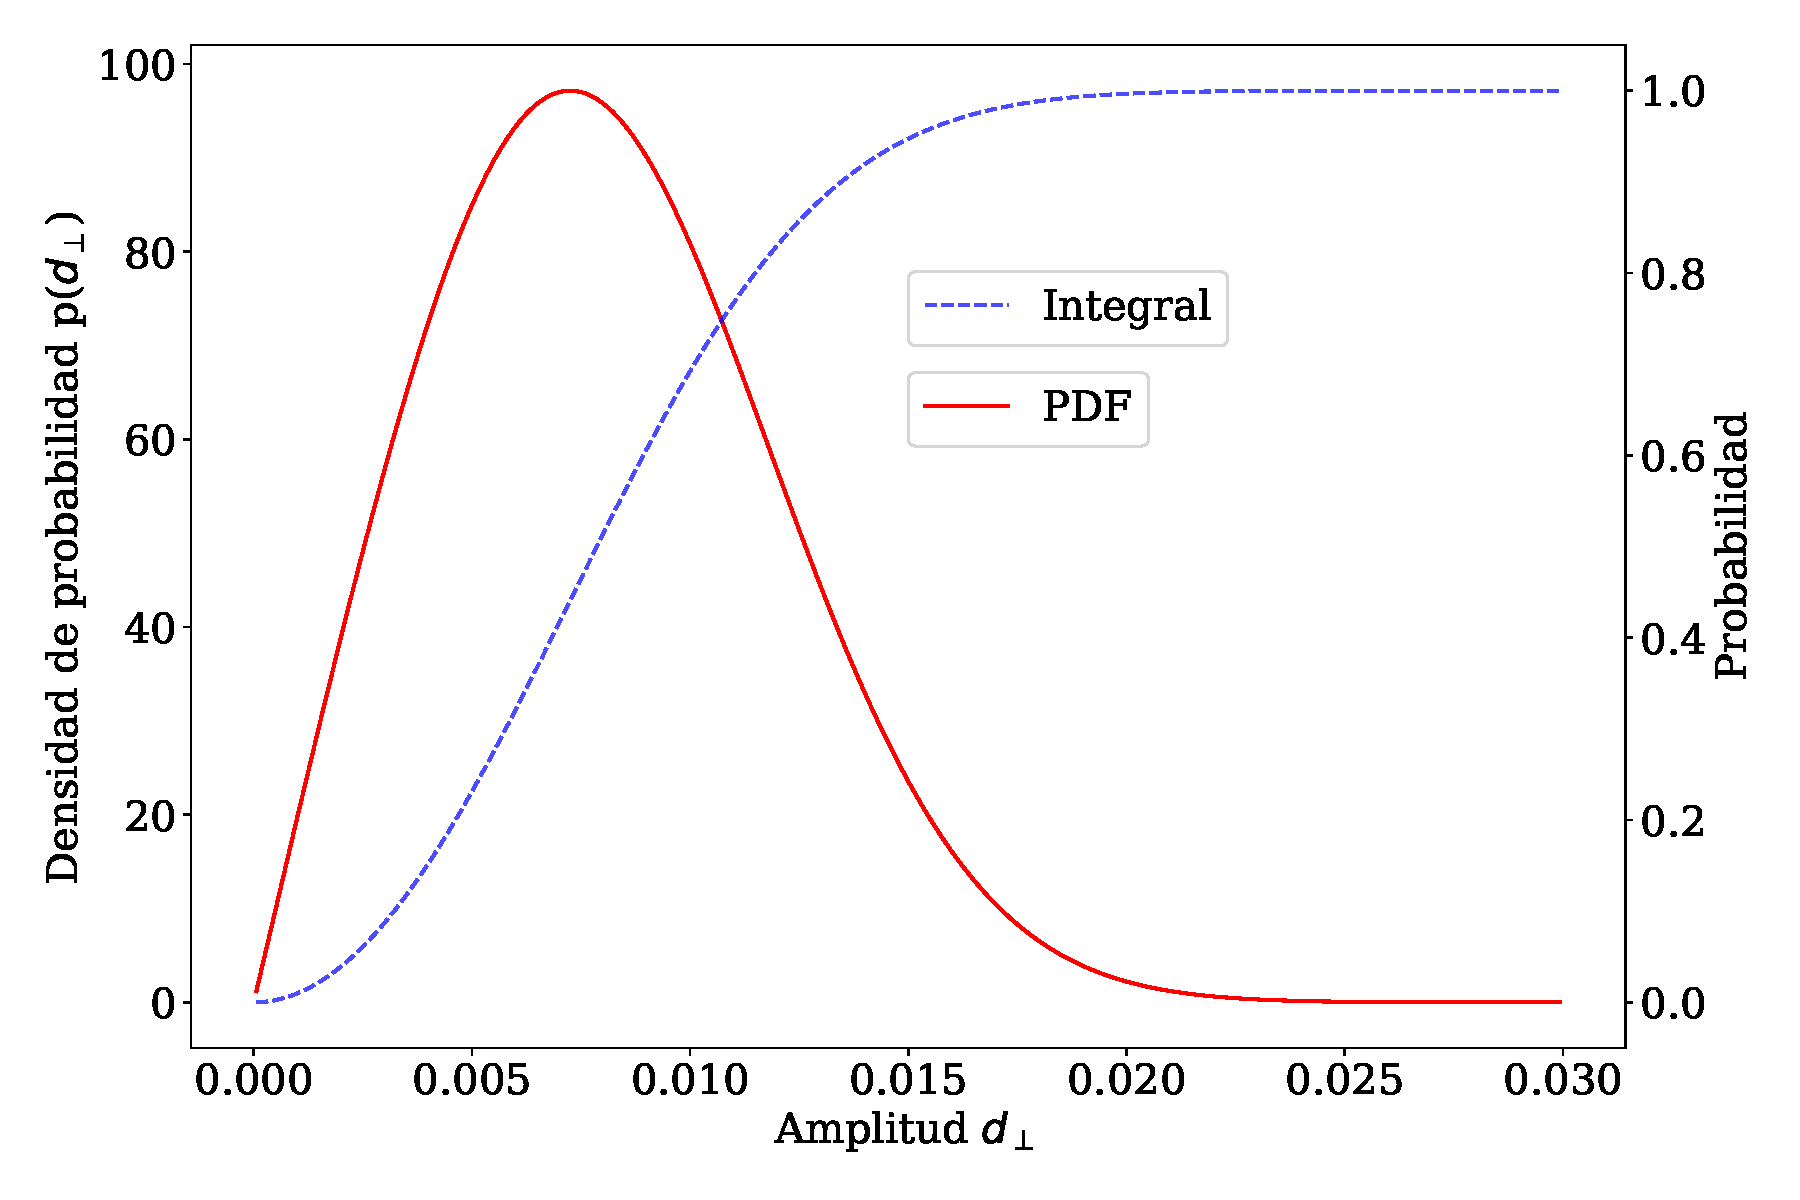
\includegraphics[width=0.75\textwidth]{bessel_prob.pdf}
        \end{center}
        \caption{}
    \end{small}
\end{figure}


\subsection{Haciendo la cuenta de los márgenes de confianza de la amplitud}

Los pasos que sigo son los siguientes: 

\begin{enumerate}
    \item Calculo la probabilidad asociada a $r_{max}=r +  10\sigma$. Dado que está tan alejada del valor de amplitud obtenida, el CL$\simeq 1$, por lo que uso este valor para normalizar  la Ec. \ref{ec:pdf} en el código.
    \item Una vez que tengo la función normalizada, finalmente hago la integral de la ecuación \ref{ec:integral} $CL(r)$ hasta un valor inicial de $r$ y el valor de la función $p(r)$.
    \begin{figure}[H]
        \begin{small}
            \begin{center}
                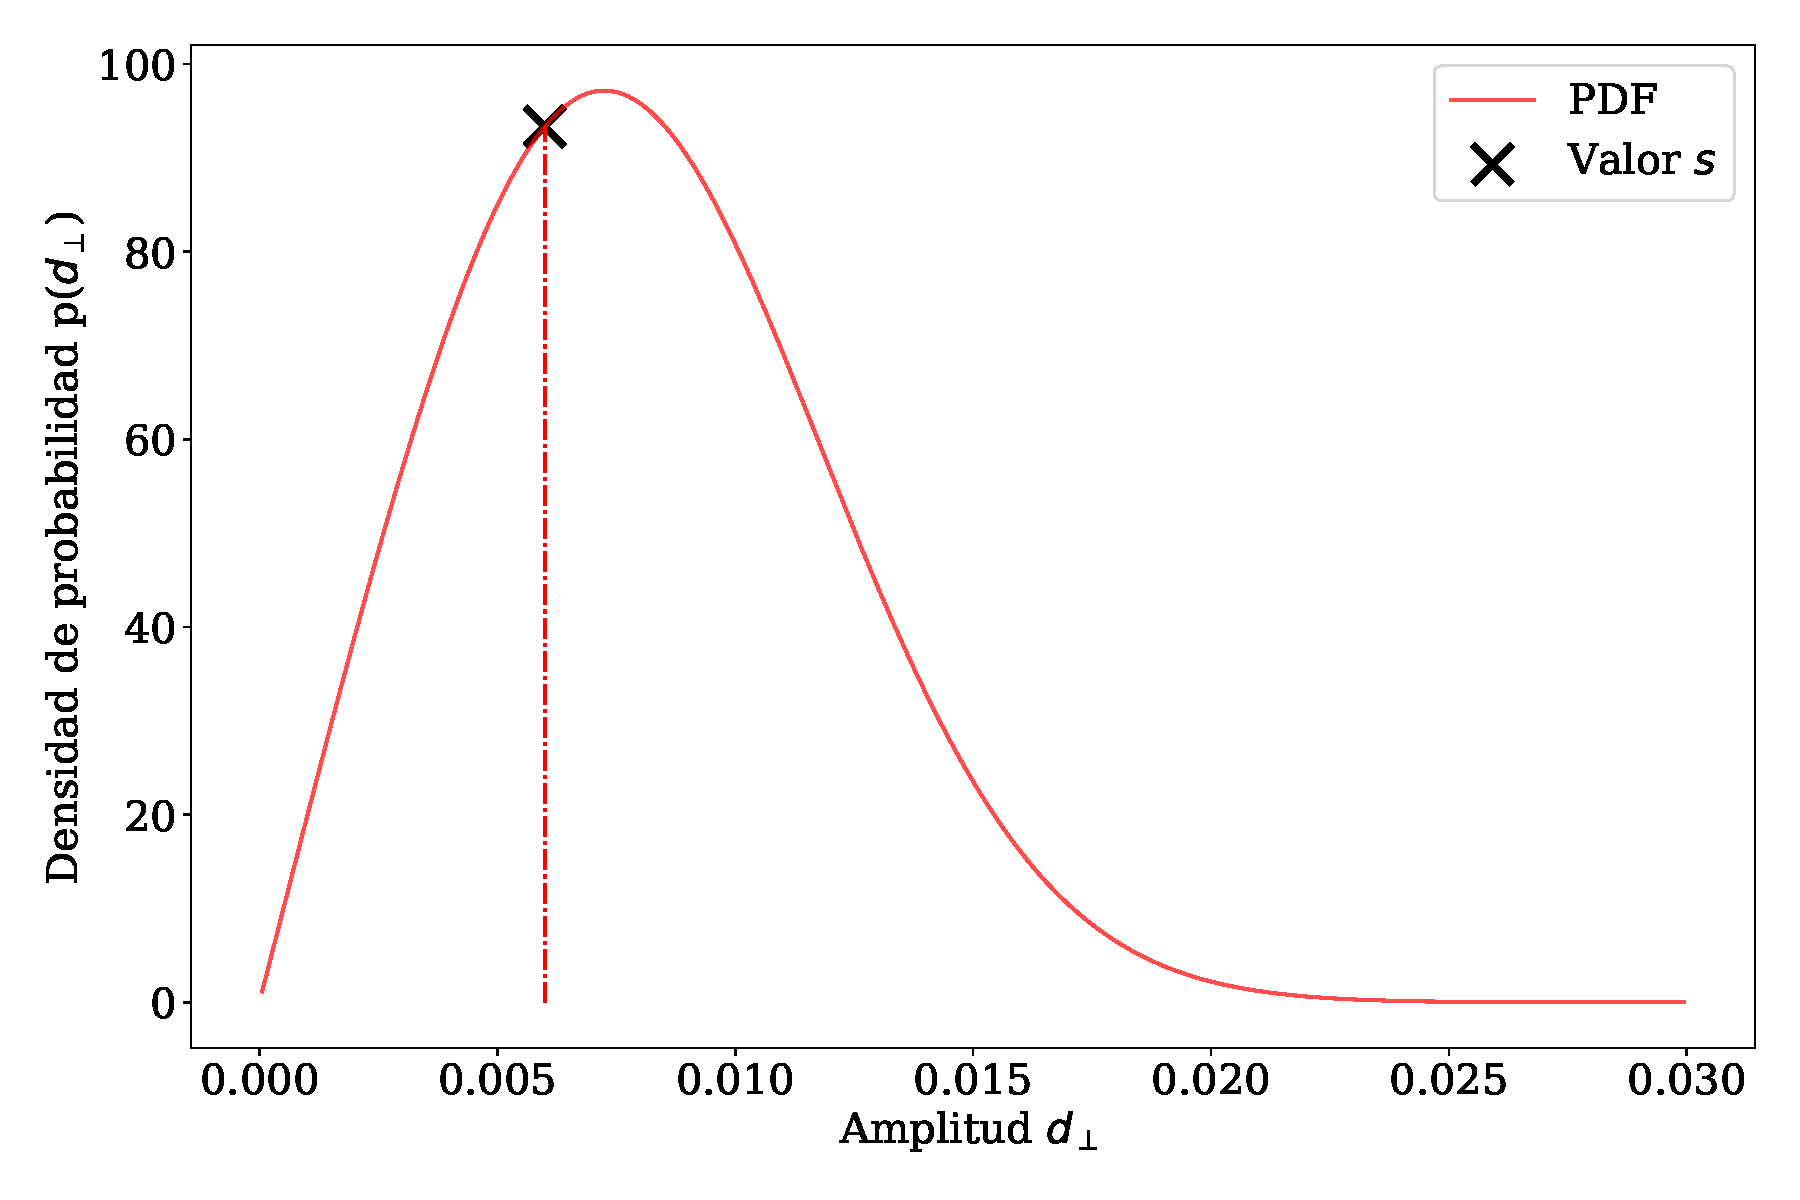
\includegraphics[width=0.75\textwidth]{bessel_prob_value_s.pdf}
            \end{center}
            \caption{}
        \end{small}
    \end{figure}
    \item Si $CL(r)< 0.683$:
    \begin{enumerate}
        \item Teniendo en cuenta el valor inicial de $p(r)_1$, se actualiza el valor  $p(r)_2 \leftarrow p(r)_1 - 0.01 p(r)_1$ \label{itm:1}.
        \item Se calcula la integral entre los dos puntos con valores igual a $p(r)_2$. 
        \item \label{itm:3} Si la integral es menor a $0.683$, se repite el proceso desde el paso \ref{itm:1}. Caso contrario, si esta integral es mayor o igual a $0.683$, se calculan los valores límites de $r$ mediante el valor $p(r)_2$ en el siguiente paso. 

        \begin{figure}[H]
            \begin{small}
                \begin{center}
                    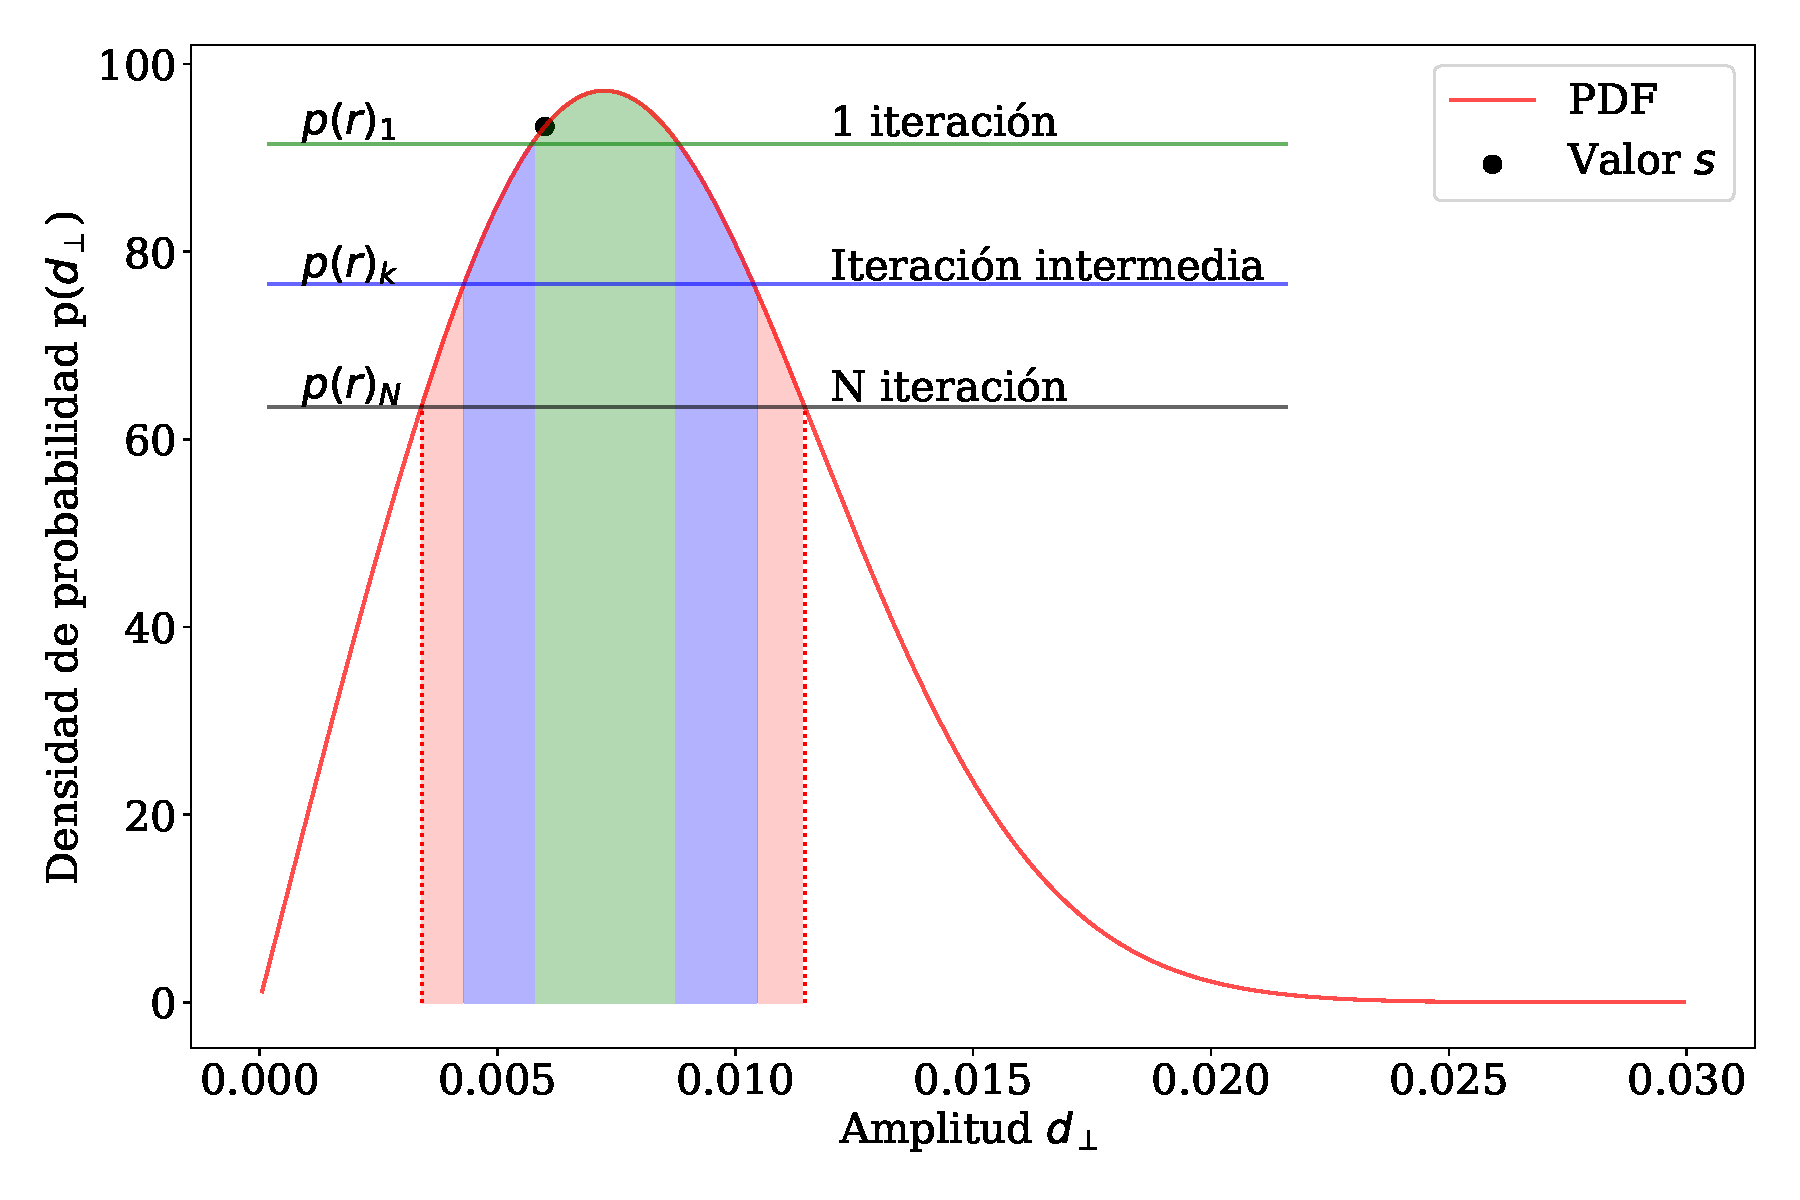
\includegraphics[width=0.75\textwidth]{bessel_prob_iterations.pdf}
                \end{center}
                \caption{}
            \end{small}
        \end{figure}



    \end{enumerate}
    \item Para calcular los límites de confianza superior $r^+$  y inferior $r^-$, teniendo en cuenta el valor final $p(r_N)$ del paso \ref{itm:3}, se calculan los valores de $r_i$ donde se cumple que $p(r_i)=p(r)_N$, los mismos son $r^+$  y  $r^-$. Finalmente los límites de confianza se calculan como:
    \begin{align*}
        \sigma^- = r-r^-\\
        \sigma^+ = r^+ -r
    \end{align*}
\end{enumerate}

\begin{figure}[H]
    \begin{small}
        \begin{center}
            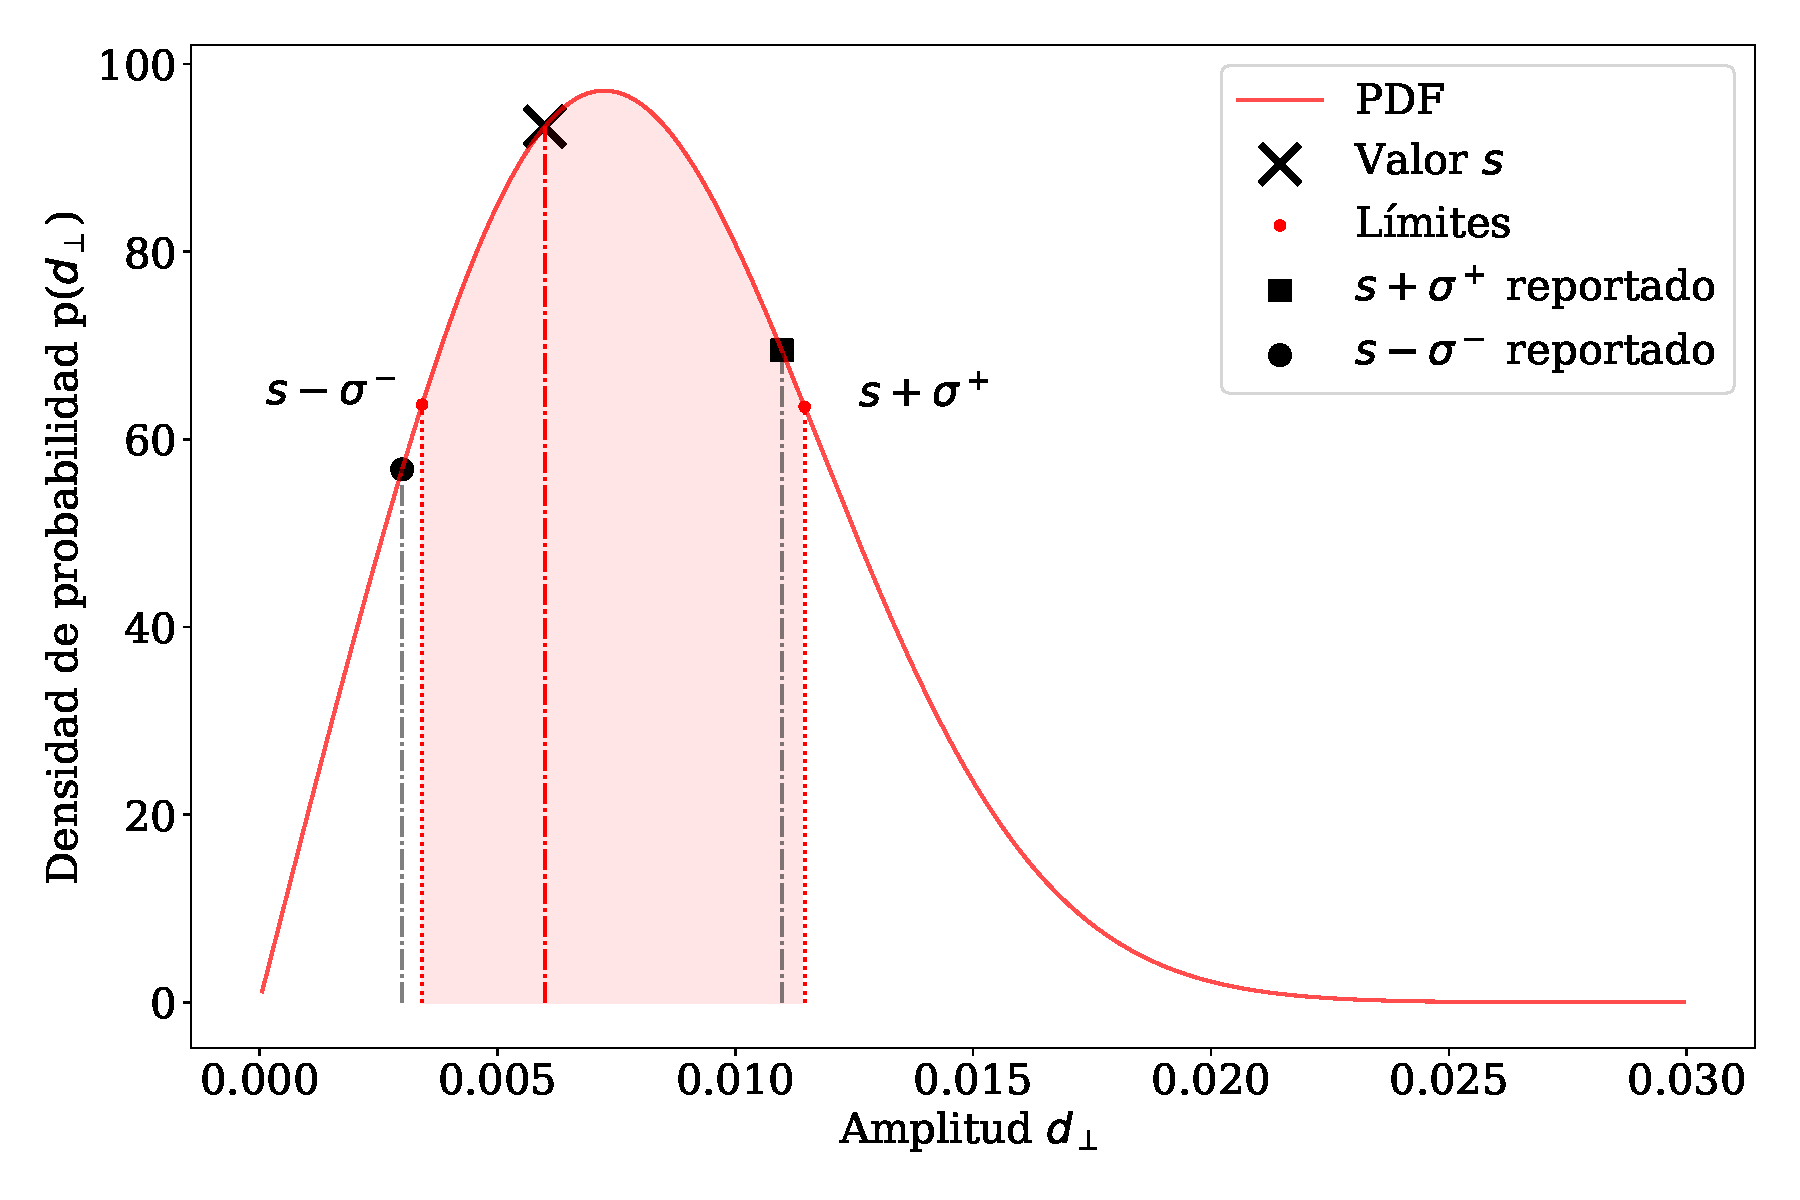
\includegraphics[width=0.75\textwidth]{bessel_prob_ej_0-25_0-5.pdf}
        \end{center}
        \caption{}
    \end{small}
\end{figure}

